\documentclass{report}

\usepackage[english]{babel}
\usepackage{emptypage}
\usepackage{lmodern}
\usepackage{microtype} 
\usepackage{graphicx}
\usepackage{tocloft}
\usepackage[latin1]{}
\usepackage{textcomp}
\usepackage{gensymb}	
\usepackage{sidecap}
\usepackage{tikz}
\usetikzlibrary{arrows,intersections}
\renewcommand{\vec}{\boldsymbol}
\usepackage{amsmath}
\usepackage{amssymb}

\usepackage{pgfplots} 
\usepackage{booktabs} 
\usepackage{tabularx} 

\usepackage{siunitx}
\usepackage{multicol,lipsum} 
\usepackage{graphicx} 
\usepackage{esvect}
\usepackage{caption}
\usepackage{subcaption}
\captionsetup{format=hang,labelfont=bf,labelsep=period}

\usepackage{mathtools}
\usepackage{float}
\usepackage{bbm}
\usepackage{amsthm}
\usetikzlibrary{arrows,intersections}
\usepackage[a4paper,top=3cm,bottom=2cm,left=2cm,right=2cm]{geometry}
\setlength{\skip\footins}{5ex plus 4pt minus 2pt}
%\renewcommand{\footnoterule}{}

\graphicspath{{images/}}

\usepackage{blkarray}
\usepackage{multirow}
\usepackage{titling}
\newcommand{\subtitle}[1]{
	\posttitle{
		\par\end{center}
	\begin{center}\large#1\end{center}
	\vskip0.5em}}
%opening

\begin{document}

\paragraph{Problem statement}
	\paragraph{Experiments preparation and data collection}

% Cenni al experiment_handler

\subsection{Mathematical description}

Il modello fisico può essere modellizzato in equazioni differenziali ordinarie (EDOs) suddividendo il sistema in singole componenti: motore DC, trasmissione, molla, massa, molla, massa. I parametri utilizzati sono i valori nominali forniti nei manuali di setup delle componenti. \\
Questa formulazione del problema può rivelarsi utile successivamente, quando il progetto del regolatore sarà basato sulla rappresentazione in spazio di stato oppure sulla funzione di trasferimento.

% \includegraphics{model}

% Immagine simulink: componenti separate

% Equazioni componenti
\begin{align*}
	V &= R_m i + L_m \frac{d}{dt}i + k_m \dot{\theta}_m \\
	\tau_m &= \eta_m k_t i , \quad \tau_{ml} = \eta_g K_g \tau_m = \eta_m \eta_g K_g k_t i \\
	J_m \ddot{\theta}_l + B_m \dot{\theta}_l &= \tau_{ml} - K_{s1} ( \theta_l - \theta_1 )
\end{align*}

\textit{Model of the 1-d.o.f. system}
\[ J_1 \ddot{\theta}_1 + B_1 \dot{\theta}_1 = K_{s_1} ( \theta_l - \theta_1 ) \]
\textit{Model of the 2-d.o.f. system}
\\
\[ J_1 \ddot{\theta}_1 + B_1 \dot{\theta}_1 = K_{s_1} ( \theta_l - \theta_1 ) - K_{s_2} ( \theta_1 - \theta_2 ) \]
\[ J_2 \ddot{\theta}_2 + B_2 \dot{\theta}_2 = K_{s_2} ( \theta_1 - \theta_2 ) \]

% Forma di stato
\textit{State-space representation of the 1-d.o.f. system}

\[
\begin{array}{ccccc}
	-\frac{R_m}{L_m} & 0 & -\frac{k_m K_g}{L_m} & 0 & 0 \\
	0 & 0 & 1 & 0 & 0 \\
	\frac{\eta_m \eta_g k_t K_g}{J_m} & -\frac{K_{s_1}}
	
\end{array}
\]

Da questa ultima formulazione matematica, è facile verificare (tramite delle funzioni \textit{ctrb} e \textit{obsv} di Matlab) la controllabilità, per mezzo della tensione applicata al motore, e l'osservabilità del sistema.
Il sistema con una sola massa rotante (1-dof) è controllabile solamente in 2 variabili di stato su 5: certamente, una di queste è la corrente (direttamente influenzata dall'input), l'altra è una a scelta tra le restanti. Viceversa, il rango della matrice di osservabilità è 4 su 5: dal momento che la corrente non è misurabile tramite un sensore, non se ne può conoscere esattamente la dinamica; al contrario, tutte le altre variabili di stato sono osservabili perché misurate. \\

Vista l'impossibilità di verificare la correttezza della dinamica di corrente tramite esperimenti, si è deciso di ignorarla~($L_m = 0$): la corrente dipende staticamente dalla tensione di input e dalla f.e.m. Riscrivendo le equazioni, otteniamo il modello ridotto:
% Forma di stato ridotta


Per poter verificare la correttezza di questo modello, si sono condotti degli esperimenti sul sistema reale, innanzitutto collegando solo la prima massa, poi entrambe.
Imponendo una tensione sul motore, si è confrontata la risposta in anello aperto del sistema fisico con la simulazione eseguita da Simulink e basata sul modello matematico.
\paragraph{Experiments input}
Gli esperimenti atti all'identificazione e validazione del modello, tutti con tensione del motore come variabile di input, sono di due tipi: scalini di varie ampiezze e sinusoidi a frequenza variabile. 
L'intervallo di tensioni applicate varia da -10V a 10V, ad intervalli di 2V (eccetto lo scalino a 0V), per un totale di 10 esperimenti.

Si è innanzitutto verificato il guadagno statico della FdT dall'input di controllo del motore alla velocità del primo carico. Imponendo una tensione costante, terminato il transitorio di assestamento della massa, si è osservato che il modello matematico sottostima la velocità di regime.
Abbiamo manualmente modificato i parametri che più inficiano il guadagno statico: la resistenza rotorica del motore, l'efficienza del motore, l'efficienza meccanica della trasmissione, la costante corrente-coppia e, infine, la costante velocità-tensione (causa della forza elettromotrice).

Dagli esperimenti, si è osservato che il comportamento del sistema non è perfettamente lineare rispetto alla tensione imposta al motore. Alcune interpretazioni fisiche sono state avanzate: l'efficienza meccanica della trasmissione, probabilmente, è sottostimata a basse velocità; per quanto riguarda la $k_m$ (causa della forza elettromotrice), una stima di tale parametro è difficile dal momento che il suo effetto contrasta la potenza del motore in modo significativo ad alte velocità, ma pressoché nullo a basse velocità.
% parametri modificati ---> G_opt

Gli esperimenti con input sinusoidale a frequenza variabile indicano un'ulteriore differenza del modello fisico osservato rispetto a quello nominale. Le oscillazioni in frequenza di risonanza del modello nominale avvengono a frequenza maggiore, anche se l'ampiezza delle oscillazioni è comparabile.


Questo fatto ha implicazioni anche nel transitorio di risposta agli scalini: la sovra-elongazione iniziale e le successive oscillazioni dipendono da poli complessi coniugati, legati ai parametri fisici delle molle e masse (costante elastica, inerzia e coefficiente di frizione). \\
Un aggiustamento del guadagno statico non permette di migliorare il comportamento del modello matematico durante il transitorio. Modificare manualmente tutti gli altri parametri sarebbe stata particolarmente gravoso, dal momento che si tratta di un approccio trial-and-error non basato su precise deduzioni razionali (il manuale di riferimento delle componenti meccaniche indica che i parametri nominali sono stati ottenuti sperimentalmente).
Una soluzione a questo problema è svincolarsi dal modello puramente matematico (white-box) e sfruttare i dati sperimentali.


\subsection{Black-box identification}

\textit{Black-box identification with a parametric method of TF in time-domain}
\\ \par Un approccio a scatola nera non tiene conto in alcun modo del modello matematico e delle sue le grandezza fisiche; al contrario, si basa esclusivamente sui dati raccolti in laboratorio tramite esperimenti.


Dal momento che questo approccio non include un significato fisico, ha senso stimare solo la FdT di nostro interesse: dalla tensione alla velocità delle masse 1 oppure 2, in funzione nel numero di dof. 
L'ordine della 





Poiché la TF vede solamente i poli osservabili e controllabili, il numero di poli imposto alla funzione di identificazione è ottenuto osservando i risultati del computer: se aggiungendo ulteriori poli, il risultato coincide con quello di un numero inferiore di poli, allora si è ottenuto l'ordine del sistema.
Con questo procedimento troviamo una TF del 3° ordine, con 2 zeri a parte reale positiva: in questo modo la perdita di fase ad alta frequenza del modello white-box e black-box coincidono. Il guadagno ad alta frequenza, però, è molto meno pendente.

Per sopperire questo problema, abbiamo deciso di imporre il numero di poli e zeri nell'identificazione: sono stati imposti uguali alla TF ottenuta nella white-box. Dunque, nel sistema con 1dof abbiamo considerato 3 poli e 0 zeri, nel sistema a 2dof 5 poli e 0 zeri.
In aggiunta ai poli del modello, va aggiunto il polo del filtro passa-basso (utilizzato per tagliare il rumore della misurazione di velocità). \\
In questo modo, sia il modulo che la fase sono molto simili a quelle del modello matematico a tutte le frequenze.

Seguendo questo approccio, si è osservato che la frequenza di risonanza del modello identificato sperimentalmente è più bassa rispetto al modello nominale; anche lo smorzamento è inferiore.
Queste difformità si sono potute osservare immediatamente anche negli esperimenti condotti in laboratorio, in particolare, con input sinusoidale a frequenza variabile.
Si ricordi che la misurazione della velocità contiene di per sè un rumore, di cui non viene tenuto conto con questa tecnica di identificazione; il filtro applicato ai dati in uscita del sensore, infatti, taglia solamente il rumore a frequenza più alta.
Pertanto, ottenere la posizione integrando la velocità stimata tramite questa FdT genererebbe un effetto di drift che incrementa con il tempo.
% scope Simulink: dati sperimentali confrontati con G_opt(DC gain aggiustato) e black-box

I dati raccolti dal sensore di velocità della massa (encoder) sono stati collezionati in un set di esperimenti tramite le funzioni Matlab \textit{iddata()} e \textit{merge()}. Il set di esperimenti così costruito è l'input della funzione \textit{tfest()}: l'output ottenuto è il modello identificato tramite approccio black-box.

\subsection{Gray-box identification}

\textit{Gray-box identification with a parametric error method of state-space time-domain}
\\ \par Il vantaggio di un approccio grey-box sta nel conservare il modello matematico e calibrare i parametri utilizzando i dati sperimentali raccolti. Il modello matematico è basato sui parametri nominali, di cui è definita anche l'incertezza (riportata nella documentazione): in questo modo, l'identificazione può tarare i ciascun parametro in un intervallo di valori ben definito e limitato, ciascuno con un significato fisico. Riguardo i parametri fisici delle masse (momento d'inerzia e coefficiente d'attrito), l'incertezza è fissata a valori tra il 10\% e 20 \%; tutti gli altri parametri hanno intervallo di incertezza come specificato sui file forniti dal produttore delle componenti.

Operativamente, abbiamo collezionato i dati di vari esperimenti e eseguito la stima del modello tramite \textit{greyest()}. Le misurazioni su cui è stata fatta l'identificazione includono sia la posizione che la velocità delle masse: questo permette di avere un set di dati di output più ampio e vario.

I risultati dell'identificazione sono molto soddisfacenti: la precisione del modello identificato rispetto ai dati di posizione è superiore al 99\%, mentre quella delle velocità superiore al 85\%. Va sottolineato che i dati utilizzati per l'identificazione contengono un rumore di misurazione, principalmente sulla velocità (in quanto derivata dalla posizione); la funzione Matlab permette anche di identificare la varianza di tale rumore, separando questo dalla dinamica del sistema. Questa è, probabilmente, anche la ragione per cui la precisione dell'identificazione sulla velocità è leggermente inferiore dell'altra.

Il modello identificato ha una pulsazione di risonanza in mezzo a quella del modello nominale e black-box;, inoltre, osservando i dati raccolti in laboratorio, si avvicina molto al sistema reale.


	
\section{Model identification}
	\subsection{Mathematical description}

The physical model can be described by ordinary differential equations (ODEs), subdividing the system into single components: DC motor, gear, first spring, first mass, second spring, second mass. The parameters used are the nominal values defined in the manuals of components setup. This formulation of the problem can be useful in the following chapters, when the controller design will depend on the state-space realization or on the transfer functions.
\begin{figure*}[h]
	\centering
	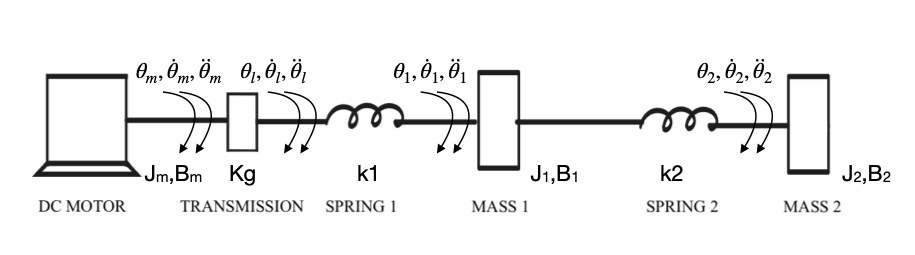
\includegraphics[width=0.8\columnwidth]{images/model/system_scheme}
	\caption{Scheme of the physical model}
\end{figure*}

% Equazioni componenti
\textit{Model of the motor and gear box}
\begin{subequations}
	\begin{align}
		V &= R_m i + L_m \frac{d}{dt}i + k_m \dot{\theta}_m \\
		\tau_m &= \eta_m k_t i \\
		\tau_{ml} &= \eta_g K_g \tau_m = \eta_m \eta_g K_g k_t i\\
		&= -J_m \ddot{\theta}_l - B_m \dot{\theta}_l - K_{s1} ( \theta_l - \theta_1 ) \qquad  \theta_l = \frac {1}{K_g} \theta_m \\
		\label{model_equations}
	\end{align}
	%\caption{Model equations}
\end{subequations}

\textit{Model of the 1 d.o.f. system}
\begin{equation}
	J_1 \ddot{\theta}_1 + B_1 \dot{\theta}_1 = K_{s_1} ( \theta_l - \theta_1 )
\end{equation}

\textit{Model of the 2 d.o.f. system}
\begin{subequations}
	\begin{align}
		J_1 \ddot{\theta}_1 + B_1 \dot{\theta}_1 &= K_{s_1} ( \theta_l - \theta_1 ) - K_{s_2} ( \theta_1 - \theta_2 ) \\
		J_2 \ddot{\theta}_2 + B_2 \dot{\theta}_2 &= K_{s_2} ( \theta_1 - \theta_2 )
	\end{align}
\end{subequations}

% Forma di stato
\textit{State-space representation of the complete 1 d.o.f. system}
\begin{equation}
	\begin{bmatrix}
		\dot{i} \\
		\dot{\theta_l} \\
		\ddot{\theta_l} \\
		\dot{\theta_1} \\
		\ddot{\theta_1}
	\end{bmatrix}
	=
	\begin{bmatrix}
		-\frac{R_m}{L_m} & 0 & -\frac{k_m K_g}{L_m} & 0 & 0 \\
		0 & 0 &1 & 0 & 0 \\
		\frac{\eta_m \eta_g k_t K_g}{J_m} & -\frac{K_{s_1}}{J_m} & -\frac{B_m}{J_m} & \frac{K_{s_1}}{J_m} & 0 \\
		0 & 0 & 0 & 0 & 1 \\
		0 & \frac{K_{s_1}}{J_1} & 0 & -\frac{K_{s_1}}{J_1} & -\frac{B_1}{J_1}
	\end{bmatrix}
	\begin{bmatrix}
		i \\
		\theta_l \\
		\theta_l \\
		\theta_1 \\
		\theta_1
	\end{bmatrix}
	+
	\begin{bmatrix}
		\frac{1}{L_m} \\
		0 \\
		0 \\
		0 \\
		0
	\end{bmatrix}
	V
\end{equation}

\textit{State-space representation of the complete 2 d.o.f. system}
\begin{equation}
	\begin{bmatrix}
		\dot{i} \\
		\dot{\theta_l} \\
		\ddot{\theta_l} \\
		\dot{\theta_1} \\
		\ddot{\theta_1} \\
		\dot{\theta_2} \\
		\ddot{\theta_2}
	\end{bmatrix}
	=
	\begin{bmatrix}
		-\frac{R_m}{L_m} & 0 & -\frac{k_m K_g}{L_m} & 0 & 0 & 0 & 0 \\
		0 & 0 &1 & 0 & 0 & 0 & 0 \\
		\frac{\eta_m \eta_g k_t K_g}{J_m} & -\frac{K_{s_1}}{J_m} & -\frac{B_m}{J_m} & \frac{K_{s_1}}{J_m} & 0 & 0 & 0 \\
		0 & 0 & 0 & 0 & 1 & 0 & 0 \\
		0 & \frac{K_{s_1}}{J_1} & 0 & -\frac{K_{s_1}+K_{s_2}}{J_1} & -\frac{B_1}{J_1} & \frac{K_{s_2}}{J_1} & 0 \\
		0 & 0 & 0 & 0 & 0 & 0 & 1 \\
		0 & 0 & 0 & \frac{K_{s_2}}{J_2} & 0 & -\frac{K_{s_2}}{J_2} & -\frac{B_2}{J_2}
	\end{bmatrix}
	\begin{bmatrix}
		i \\
		\theta_l \\
		\theta_l \\
		\theta_1 \\
		\theta_1 \\
		\theta_2 \\
		\theta_2
	\end{bmatrix}
	+
	\begin{bmatrix}
		\frac{1}{L_m} \\
		0 \\
		0 \\
		0 \\
		0 \\
		0 \\
		0
	\end{bmatrix}
	V
\end{equation}

From this mathematical formulation, it is easy to check (thanks to Matlab functions  \textit{ctrb} e \textit{obsv}) the controllability by means of the voltage applied to the motor and the system observability.
The system having just one rotating mass (i.e. 1 d.o.f. system) is controllable only in two state variables over five: surely, one of those is the current (directly affected by the input), the other is one among the remaining. On the other hand, the observability matrix~$M_O$ is full rank; however, it must be considered that the current~$i$ dynamics is extremely rapid (the time constant is defined as~$\tau_i = \frac{L_m}{R_m} = 7.56\ 10^-5 \ s$), then the sampling time~($T_s = 2 ms$) prevents its observation even with a current sensor installed on the motor.
Similarly to this case, it can be expected that also the 2 d.o.f. system is not fully controllable. \\

Since the current dynamics cannot be verified by experimental data, we have decided to ignore it~(the rest of the model is not significantly affected by that, since its transient is definitely negligible): in the following model, the current statically depends on the input voltage and the electromotive force (back-emf).
% Forma di stato ridotta
\textit{State-space representation of the reduced 1 d.o.f. system}
\begin{equation}
	\begin{bmatrix}
		\dot{\theta_l} \\
		\ddot{\theta_l} \\
		\dot{\theta_1} \\
		\ddot{\theta_1}
	\end{bmatrix}
	=
	\begin{bmatrix}
		0 &1 & 0 & 0 \\
		-\frac{K_{s_1}}{J_m} & -\frac{B_m}{J_m}-\frac{\eta_m \eta_g k_t k_m {K_g}^2}{R_m J_m}  & \frac{K_{s_1}}{J_m} & 0 \\
		0 & 0 & 0 & 1 \\
		\frac{K_{s_1}}{J_1} & 0 & -\frac{K_{s_1}}{J_1} & -\frac{B_1}{J_1}
	\end{bmatrix}
	\begin{bmatrix}
		\theta_l \\
		\theta_l \\
		\theta_1 \\
		\theta_1
	\end{bmatrix}
	+
	\begin{bmatrix}
		0 \\
		\frac{\eta_m \eta_g k_t K_g}{R_m J_m} \\
		0 \\
		0
	\end{bmatrix}
	V
\end{equation}

\textit{State-space representation of the reduced 2 d.o.f. system}
\begin{equation}
	\begin{bmatrix}
		\dot{\theta_l} \\
		\ddot{\theta_l} \\
		\dot{\theta_1} \\
		\ddot{\theta_1} \\
		\dot{\theta_2} \\
		\ddot{\theta_2}
	\end{bmatrix}
	=
	\begin{bmatrix}
		0 &1 & 0 & 0 & 0 & 0 \\
		-\frac{K_{s_1}}{J_m} & -\frac{B_m}{J_m}-\frac{\eta_m \eta_g k_t k_m {K_g}^2}{R_m J_m}  & \frac{K_{s_1}}{J_m} & 0 & 0 & 0 \\
		0 & 0 & 0 & 1 & 0 & 0 \\
		\frac{K_{s_1}}{J_1} & 0 & -\frac{K_{s_1}+K_{s_2}}{J_1} & -\frac{B_1}{J_1} & \frac{K_{s_2}}{J_1} & 0 \\
		0 & 0 & 0 & 0 & 0 & 1 \\
		0 & 0 & \frac{K_{s_2}}{J_2} & 0 & -\frac{K_{s_2}}{J_2} & -\frac{B_2}{J_2}
	\end{bmatrix}
	\begin{bmatrix}
		\theta_l \\
		\theta_l \\
		\theta_1 \\
		\theta_1 \\
		\theta_2 \\
		\theta_2
	\end{bmatrix}
	+
	\begin{bmatrix}
		0 \\
		\frac{\eta_m \eta_g k_t K_g}{R_m J_m} \\
		0 \\
		0 \\
		0 \\
		0
	\end{bmatrix}
	V
\end{equation}
This time, checking again the controllability and observability of the reduced order system, matrices~$M_R$ e $M_O$ are full rank. \\

In order to validate this model, some experiments on the real system have been performed. Firstly, only one mass and, then, two masses in cascade were linked to the shaft. By imposing to the motor a certain voltage, the open-loop response has been compared to the Simulink simulation (based on the model previously illustrated).

\paragraph{Experiments input}
The experiments aimed at identifying and validating the model, all performed by imposing a voltage to the motor, can be classified into two types: steps (multiple in time and of different size) and variable frequency sine waves. The range of applied voltages~($\pm 10\ V$) is constrained by the motor physical limitations.

Firstly, the static gain of the transfer function between the control input of the motor and the first mass speed~($G_{V,\dot{\theta}_1}$) has been checked. To do this, a constant voltage has been imposed; once the transient of first mass settlement is over, it is clear that the mathematical model underestimates the steady-state speed.
So, we have initially changed the model parameters whose effect on the static gain is more significant: the rotor resistance~($R_m$), the motor efficiency~($\eta_m$), the mechanical efficiency of the gear~($\eta_g$), the current-torque constant~($k_t$) and the mass speed-voltage constant (~$k_m$, responsible of the back-emf).

Thanks to the experiments, it has been noticed that the real system behavior is not exactely linear with respect to the imposed voltage. Some physical interpretations have been proposed: the mechanical efficiency of the gear~($\eta_g$) is probably underestimated at low speeds; then, the~$k_m$ constant (that generates the back-emf), is very difficult to be estimated, since its effect on the motor power is quite significant at high speed, but almost negligible at low speed.

% parametri modificati ---> G_opt

The variable frequency sine wave experiments suggest another significant difference between the physical model and the nominal one. Here, it is visible that resonance frequency of the nominal model is greater that the real one; anyway, the amplitude of the oscillations at those frequencies is comparable. \\
This fact affects also the step response transient: the initial overshoot and later oscillations depend on complex conjugate poles, linked to the physical parameters of springs and masses (spring stiffness~$K_s$, mass inertia~$J$, mass friction coefficient~$B$). \\

A tuning of the static gain does not allow an improvement of the mathematical model in the transient behavior. However, manually changing all the other parameters would be particularly difficult, since it is a trial-and-error approach based on no precise rational reasoning (it must be considered also, indeed, that nominal parameters shown in the reference manual are obtained experimentally).
A solution to this problem is to untie our approach from the purely mathematical model (i.e. white-box) and use experimental data.

\subsection{Black-box identification}

\textit{Black-box identification with a parametric method of TF in time-domain} \\

\par A black-box approach totally loses a connection to the mathematical model and its physical dimensions; on the contrary, it is exclusively based on data collected by experiments in laboratory.
For this reason, it is reasonable to estimate only the transfer function of our interest (according to the design of the controller of speed, designed later):~$G_{V,\dot{\theta_1}}$ or~$G_{V,\dot{\theta_2}}$, meaning the transfer functions from the voltage (input) and the masses speed. \\

Masses speeds (generated by the derivation of encoder data) are collected in a set of experiments by using the Matlab functions~\textit{iddata()} e~\textit{merge()}. So, the obtained data are the input of the~\textit{tfest()} function: the obtained output is the identified black-box model. \\

Remembering that the transfer function only sees observable and controllable poles, a first method to impose the number of poles in the identification function is looking at the computer results: if the obtained transfer function does not change by adding more poles, then it has been obtained the order of the system.
By this procedure, we have found a~$3^{rd}$ order transfer function, with 2 positive-real part zeros: in this way, the phase loss at high frequency of the nominal and empirical models coincide. On the other hand, the gain at that frequency is much less inclined.

\begin{figure*}[h]
	\centering
	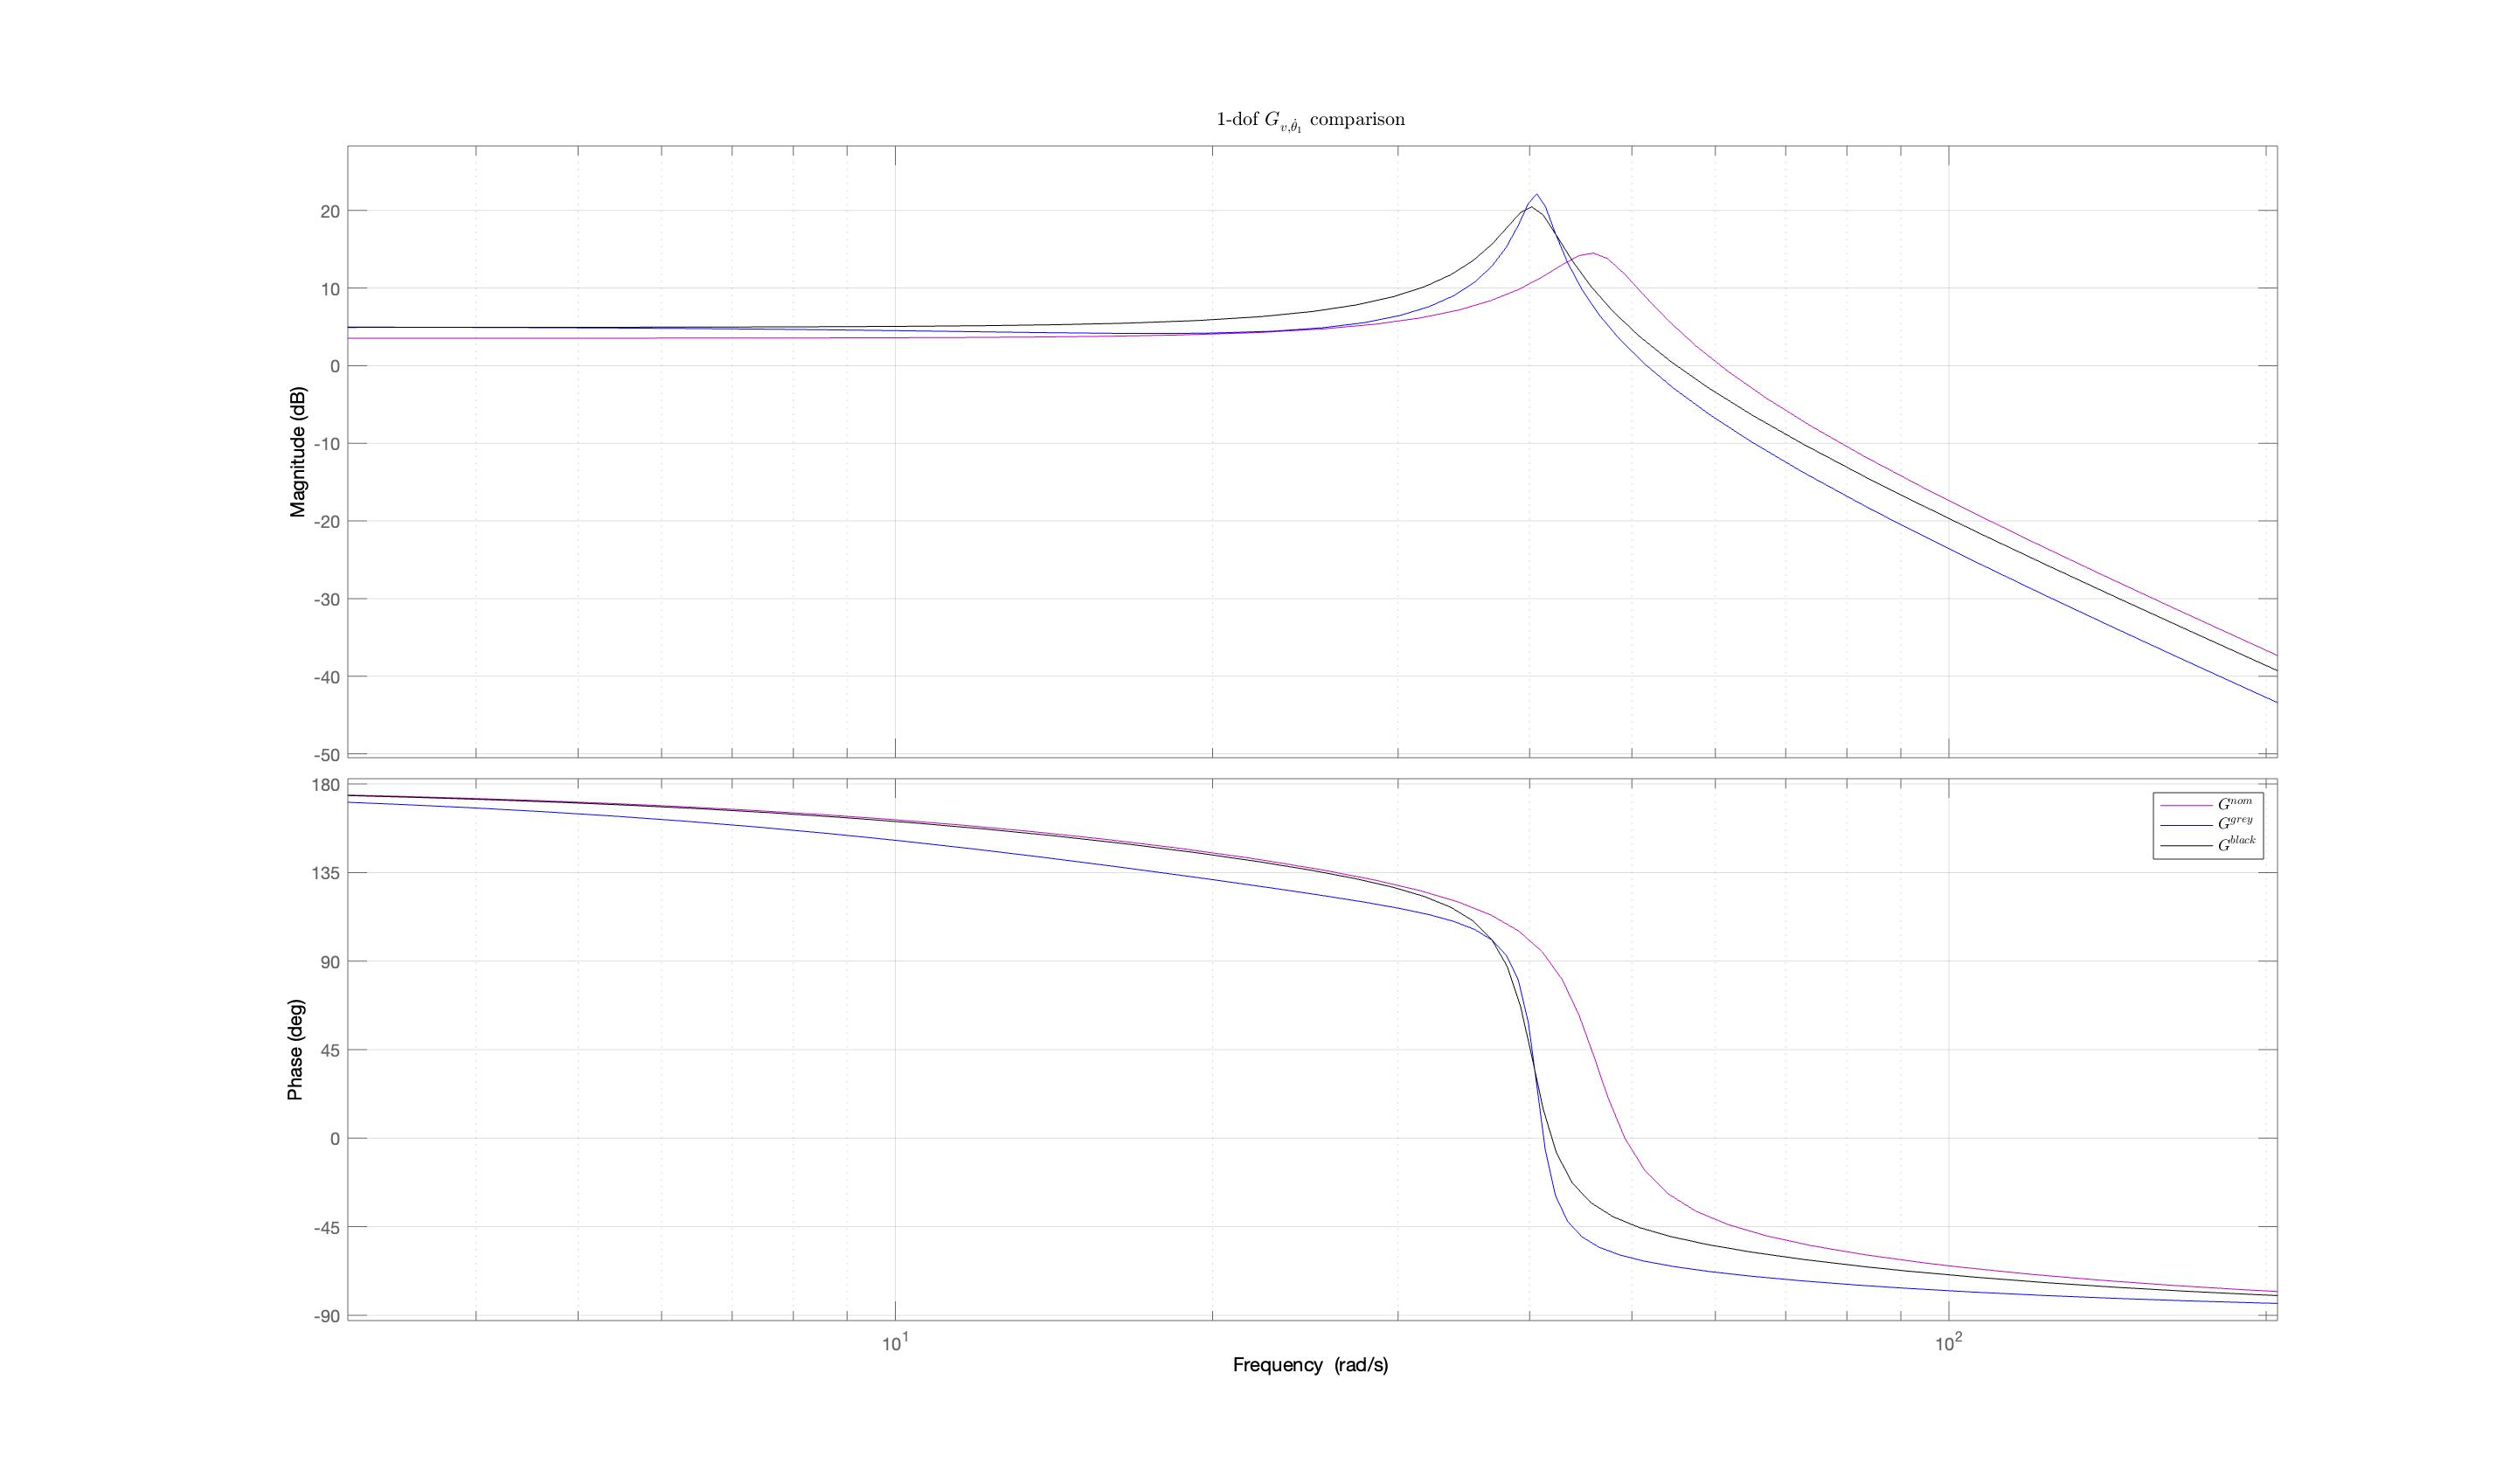
\includegraphics[width=\columnwidth]{images/model/1dof_g_v_w1}
	\caption{1-dof system. Transfer functions comparison}
\end{figure*}

\begin{figure*}[h]
	\centering
	\begin{subfigure}{\columnwidth}
		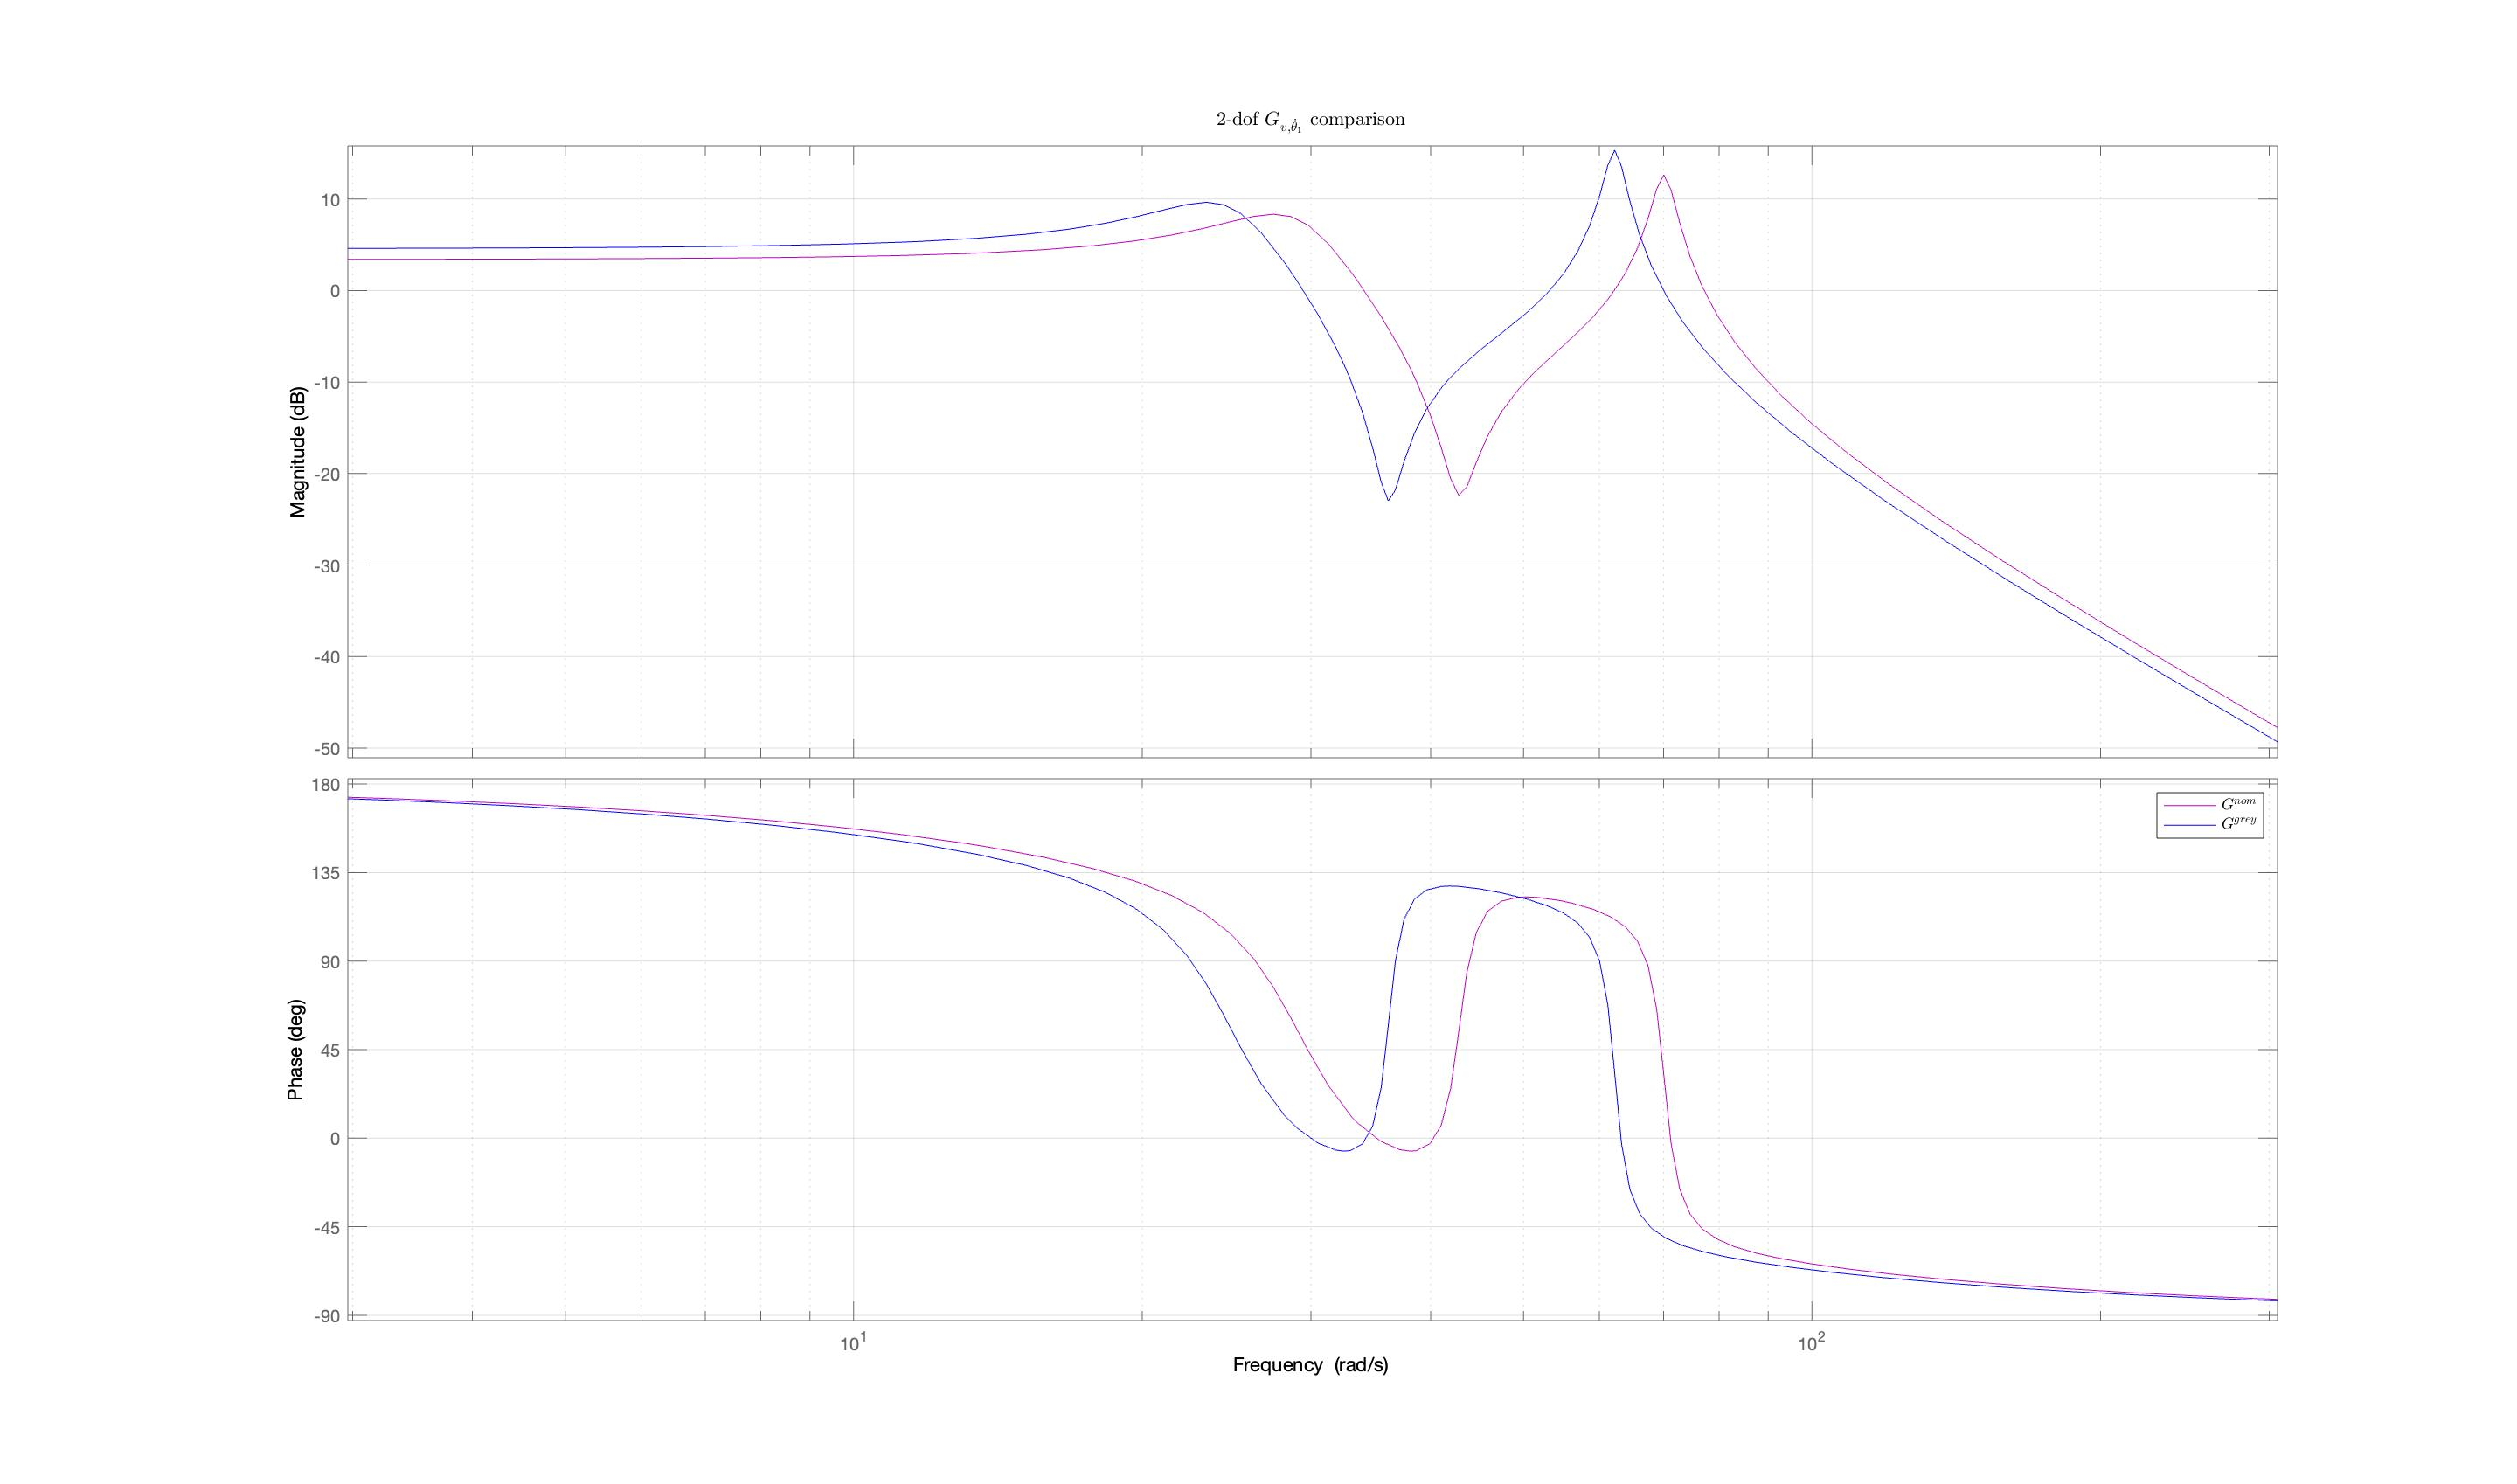
\includegraphics[width=\columnwidth]{images/model/2dof_g_v_w1}
	\end{subfigure}
	\begin{subfigure}{\columnwidth}
		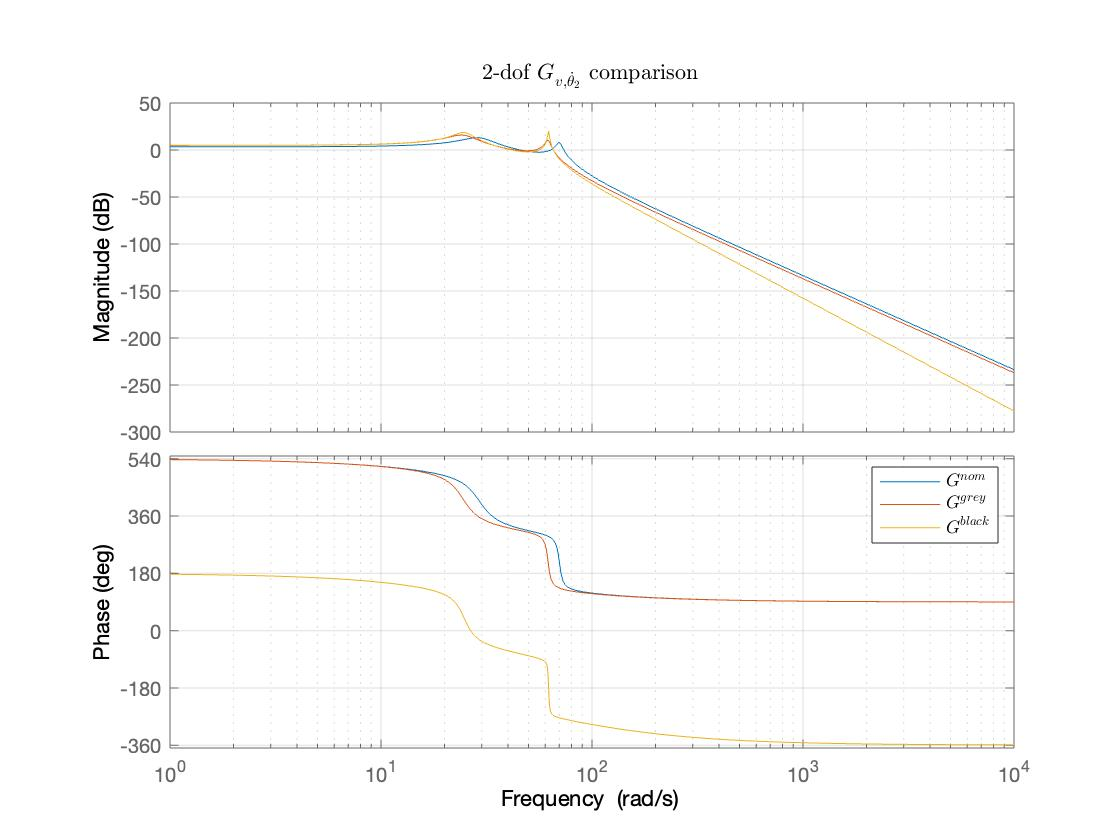
\includegraphics[width=\columnwidth]{images/model/2dof_g_v_w2}
	\end{subfigure}
	\caption{2-dof system. Transfer functions comparison}
\end{figure*}

To overcome this problem, we have decided to impose the number of both poles and zeros, that is equal to the transfer function structure computed from the white-box model. Therefore, the 1 dof system has 3 poles and 0 zeros, while the 2 dof system has 5 poles and 0 zeros.
In addition to the physical model poles, it must be considered the low-pass filter for the speed measurement noise. \\
In this way, both module and phase Bode diagrams are very similar to the mathematical ones at every frequency.

Following this approach, it has been observed that the resonance frequency of the identified model is lower that the nominal one, as the damping too.
Those differences can be immediately seen is the laboratory experiments: in particular, the ones with variable frequency sine wave. \\
It is important to remember that the speed measurement is noisy (the filter acts at very high frequency), because of the derivation from the encoder data. Hence, obtaining the position, by integrating the speed estimated by this model, would generate a drift that increases in time. \\

% scope Simulink: dati sperimentali confrontati con G_opt(DC gain aggiustato) e black-box

\subsection{Gray-box identification}

\textit{Gray-box identification with a parametric error method of state-space time-domain} \\
\par The advantage of using a gray-box approach is that it maintains the mathematical model structure and tunes parameters based on experimental data. The starting model is defined on the nominal parameters (as illustrated in Paragraph "Mathematical description"), whose uncertainties are a-prior specified: in this way, the identification can change parameters in a well defined and constrained range, preserving a physical meaning. Specifically, masses parameters (inertia~$J$, friction~$B$) uncertainty is fixed to ranges between~$10 \%$ and~$20 \%$; all the other parameters have an uncertainty range specified according to the reference manuals.
% table: nominal and identified parameters

Operatively, we have collected all data experiments and estimated the model by means of the function~\textit{greyest()}. The used measurements include both position and speed of the masses: this allows to have a larger and differentiated set of data.

Identification results are very satisfactory: the precision of the model with respect to the position data is greater that~$99 \%$, while the velocity one is about~$85 \%$. It must be remembered that all data are affected by a noise, in particular the speed ones; about this, the Matlab function allows also to identify those noises, so that they can be separated from the dynamical model.

The identified model has a resonance frequency located in between the nominal and black-box ones, as expected. Moreover, data collected in laboratory are very close to the simulation performed by using this identified model.


\end{document}